\documentclass{article}
\usepackage{enumerate}
\usepackage{amsmath}
\usepackage{amssymb}
\usepackage{graphicx}
\usepackage{subfigure}
\usepackage{geometry}
\usepackage{color}
\usepackage{bm}
\usepackage{indentfirst}
\usepackage{float}
\usepackage{booktabs}

\begin{document}

\vspace*{0.25cm}

\hrulefill

\thispagestyle{empty}

\begin{center}
\begin{large}
\sc{UM--SJTU Joint Institute \vspace{0.3em} \\ Physics Laboratory \\(VP241)}
\end{large}

\hrulefill

\vspace*{5cm}
\begin{Large}
\sc{{Laboratory Report}}
\end{Large}

\vspace{2em}

\begin{large}
\sc{{Exercise 5
\vspace{0.5em}

RC, RL, and RLC Circuits
}}
\end{large}
\end{center}


\vfill

\begin{table}[h!]
\flushleft
\begin{tabular}{lll}
Name: Yihao Liu \hspace*{2em}&
ID: 515370910207\hspace*{2em}& Group: 7\\


\\

Date: 28 Oct 2016 

\end{tabular}
\end{table}

\hfill
\begin{tiny}
[rev. 1.0]
\end{tiny}

\newpage

\tableofcontents

\newpage

\section{Objectives}

The objective of this exercise is to understand the physics of alternating-current circuits, in particular the processes of charging/discharging of capacitors, the phenomenon of electromagnetic induction in inductive elements, and other dynamic processes in RC, RL, and RLC series circuits. Moreover, methods for measuring the amplitude-frequency and the phase-frequency characteristics of RC, RL, and RLC series circuits will be studied. The resonance frequency of a RLC circuit as well as the quality factor of the circuit will be found from the amplitude-frequency curve.

\section{Theoretical Background}

Resistors, capacitors, and inductors are basic elements of electric circuits. Depending
on a particular arrangement of these elements, RC, RL, RLC alternating-current (AC)
circuits may display various features, including transient, steady state, and resonant behavior.

\subsection{Transient Processes in RC, RL, RLC Series Circuits}

\subsubsection{RC Series Circuits}

In a RC circuit, the process of charging or discharging of the capacitor is an example of a transient process. Figure 1 shows a RC series circuit in which a square-wave signal is used as the source signal. In the first half of the cycle, the square-wave voltage is $ U(t) = \mathcal{E} $. and it charges the capacitor. In the second half-cycle, the square-wave voltage is zero, and the capacitor discharges through the resistor. The loop equation (Kirchhoff's loop rule) for the charging process is
\begin{equation}
	RC\dfrac{dU_C}{dt}+U_C=\mathcal{E}
\end{equation}

With the initial condition $ U_C(t = 0) = 0 $, the solution of Eq. (1) can be found as
$$ U_C=\mathcal{E}(1-e^{-\frac{t}{RC}})\text{ and } U_R=iR=\mathcal{E}e^{-\frac{t}{RC}} $$

\begin{figure}[H]
	\centering
	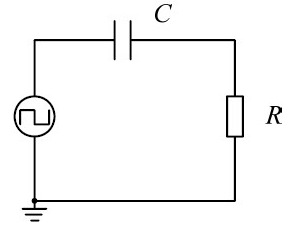
\includegraphics[scale=0.6]{fig1.jpg}
	\caption{RC series circuit.}
\end{figure}

Hence the voltage across the capacitor $ U_C $ increases exponentially with time $ t $, whereas the voltage on the resistor $ U_R $ decreases exponentially with time. The curves $ U(t),\ U_C(t), $ and $ U_R(t) $ are shown in Figure 2.

\begin{figure}[H]
	\centering
	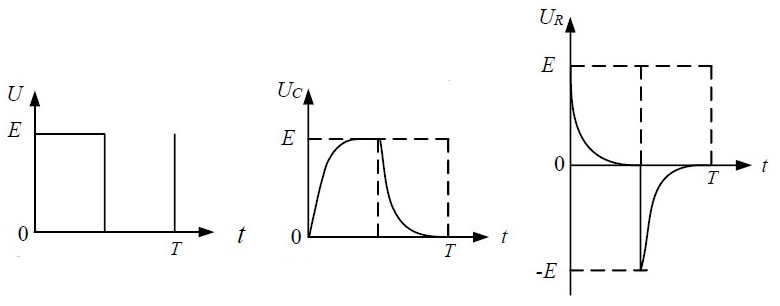
\includegraphics[scale=0.6]{fig2.jpg}
	\caption{Charging/discharging curves for a RC series circuit.}
\end{figure}

For the discharging process, the loop rule gives
\begin{equation}
	 RC\dfrac{dU_C}{dt}+U_C=0
\end{equation} 

The solution of Eq. (2), with the initial condition $ U_C(t = 0) = \mathcal{E} $, is
$$ U_C=\mathcal{E}e^{-\frac{t}{RC}} $$
and, consequenctly,
$$ U_R=iR=-\mathcal{E}e^{-\frac{t}{RC}} $$

where the magnitudes of both $ U_C $ and $ U_R $ decrease exponentially with time. Since $ RC =\tau $ has the units of time, it is called the time constant of the circuit, and characterizes the dynamics of the transient process. There is another characteristics related to the time constant, easier to measure in experiments, which is called the half-life period $ T_{1/2} $. The half-life period is the time needed for $ U_C $ to decrease to a half of the initial value (or increase to a half of the terminal value), and may be also used to characterize the dynamics of the transient process. Both quantities, in the process with exponential dynamics discussed above, are related by the equation
$$ T_{1/2}=\tau ln2\approx0.693\tau $$

\subsubsection{RL Series Circuit}
A similar analysis can be carried out for a RL series circuit. In this case,
$$ \tau=\dfrac{L}{R}\quad\text{and}\quad T_{1/2}=\dfrac{L}{R}ln2 $$

\subsubsection{RLC Series Circuit}
For the situation that a power source is suddenly plugged into a RLC
circuit, follow the loop rule we have
\begin{equation}
	LC\dfrac{d^2U_C}{dt^2}+RC\dfrac{dU_C}{dt}+U_C=\mathcal{E}
\end{equation}
both sides of the equation by LC and introducing the symbols \begin{equation}
	\beta=\dfrac{R}{2L} \text{ and } \omega_0=\dfrac{1}{\sqrt{LC}}
\end{equation}

Eq. (3) can be rewritten as
\begin{equation}
	\dfrac{d^2U_C}{dt^2}+2\beta\dfrac{dU_C}{dt}+\omega_0^2U_C=\omega_0^2\mathcal{E}
\end{equation}

Note that Eq. (5) is an inhomogeneous differential equation and it is mathematically equivalent to the equation of motion of a damped harmonic oscillator with a constant driving force. Therefore, the complementary homogeneous equation is fully analogous to the equation of motion of a damped harmonic oscillator, with $ \beta $ being the damping coefficient, and $ \omega_0 $ - the natural angular frequency. Moreover, after a specific solution to the inhomogeneous equation is found, a unique solution to the initial value problem consisting of Eq. (5) and the initial conditions
\begin{equation}
	U_C(t=0)=0 \text{ and } \left.\dfrac{dU_C}{dt}\right|_{t=0}=0
\end{equation}
can be found.
Exactly as for mechanical oscillations, depending on the relation between $ \beta $ and $ \omega_0 $, there are three regimes, as implied by the solution of the complementary homogeneous equation:

\begin{enumerate}[$\blacktriangleright$]
	\item
	If $ \beta^2-\omega_0^2<0 $ (weak damping), the system is in the underdamped regime and the solution to the initial value problem is of the form
	$$ U_C=\mathcal{E}-\mathcal{E}e^{-\beta t}\left( cos\omega t+\dfrac{\beta}{\omega}sin\omega t \right) $$
	where $ \omega=\sqrt{\omega_0^2-\beta^2} $
	\item
	If $ \beta^2-\omega_0^2>0 $ (strong damping), the system is in the overdamped regime with the	solution of the form
	$$  U_C=\mathcal{E}-\dfrac{\mathcal{E}}{2\gamma}e^{-\beta t}[(\beta+\gamma)e^{\gamma t}-(\beta-\gamma)e^{-\gamma t}]  $$
	where $ \gamma=\sqrt{\beta^2-\omega_0^2} $
	\item
	If $ \beta^2-\omega_0^2=0 $ the system is said to be critically damped, and
	\begin{equation}
		U_C=\mathcal{E}-\mathcal{E}(1+\beta t)e^{-\beta t}
	\end{equation}
\end{enumerate}

When the circuit reaches a steady state, the power source is suddenly removed. The differential equation for the discharging process is similar to that of the charging process, and there are also three regimes of the process.\\

The above discussion is valid for an ideal circuit and a step-signal source with zero internal resistance. In the experiment, the ideal system is replaced by a square-wave source with a small internal resistance. The period of the square-signal must be much greater than the time constant of the circuit. Note that, according to the above equations, the voltage across the capacitor $ U_C $ will finally reach $ \mathcal{E} $ regardless of the regime (Figure 3).

\begin{figure}[H]
	\centering
	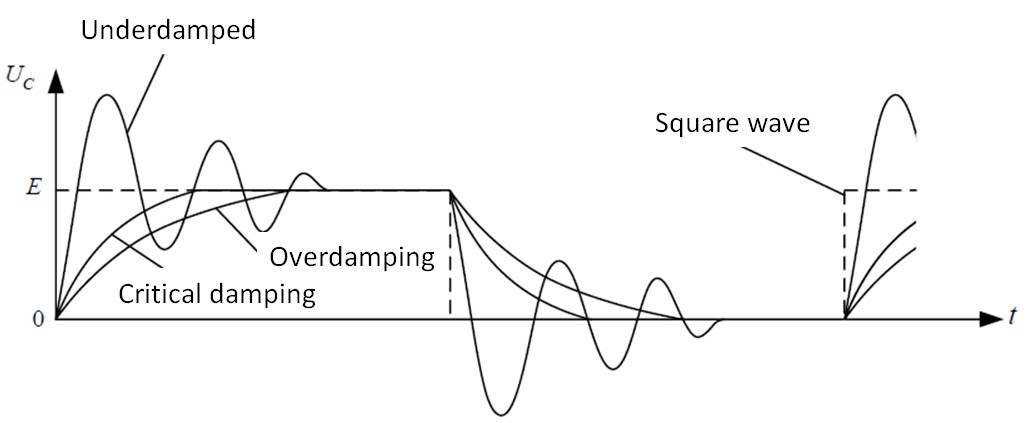
\includegraphics[scale=0.4]{fig3.jpg}
	\caption{Three different regimes of transient processes in a RLC series circuit.}
\end{figure}

\subsection{RC, RL Steady-State Circuits}
When a sinusoidal alternating input voltage is provided to a RC (or RL) series circuit, the amplitude and the phase of the voltage across the capacitor and the resistor will change with the frequency of the input voltage. Then the amplitude vs. frequency relation and the phase vs. frequency relation can be obtained by measuring the voltage across the elements in the circuit for different input signal frequencies
$$ \varphi=tan^{-1}\left(\dfrac{U_L}{U_R}\right)=tan^{-1}\left(\dfrac{\omega L}{R}\right),\qquad \varphi=tan^{-1}\left(-\dfrac{U_C}{U_R}\right)=tan^{-1}\left(-\dfrac{1}{\omega RC}\right) $$

\subsection{RLC Resonant Circuit}

\subsubsection{RLC Series Circuit}
A generic RLC series circuit is shown in Figure 4. The impedance and the phase difference in the RLC circuit can be calculated, e.g., by using the phasors technique. Representing the current I by a vector along the horizontal axis, the phase differences between the current and the voltages across the resistor, coil, and capacitor are
$$ \varphi_R=0,\qquad \varphi_L=\dfrac{\pi}{2},\qquad \varphi_C=-\dfrac{\pi}{2} $$
respectively. The corresponding voltage amplitudes across the elements are
$$ U_R=IZ=IR,\qquad U_L=IZ_L=I\omega L,\qquad U_C=IZ_C=\dfrac{I}{\omega C} $$

\begin{figure}[H]
	\centering
	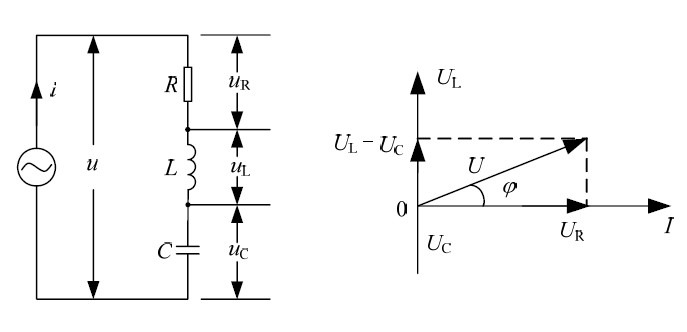
\includegraphics[scale=0.6]{fig4.jpg}
	\caption{RLC series circuit.}
\end{figure}

Hence, the voltage amplitude
\begin{equation}
	U=\sqrt{U_R^2+(U_L-U_C)^2} \text{ or } U=I\sqrt{R^2+\left(\omega L-\dfrac{1}{\omega C}\right)^2}
\end{equation}
and the total impedance
\begin{equation}
	 Z=\sqrt{R^2+\left(\omega L-\dfrac{1}{\omega C}\right)^2}
\end{equation}
with the phase difference between the current and the voltage in the circuit
$$ \varphi=tan^{-1}\left(\dfrac{U_L-U_C}{U_R}\right)=tan^{-1}\left(\dfrac{\omega L-\frac{1}{\omega C}}{R}\right) $$

\subsubsection{Resonance}
If the frequency of the input signal provided by the source satisfies the condition
$$ \omega_0 L=\dfrac{\omega}{C},\qquad \text{ or, equivalently, }\qquad \omega_0=\dfrac{1}{\sqrt{LC}} $$
the total impedance will reach a minimum, $ Z_0 = R $. Note that the resistance R in a real circuit includes the internal resistance and all kinds of alternating-current power losses, so its actual value will be greater than the theoretical one.\\

When the current reaches its maximum, $ I_m = U/R $, the circuit is said to be at resonance. The frequency
$$ f_0=\dfrac{\omega_0}{2\pi}=\dfrac{1}{2\pi\sqrt{LC}} $$
at which the resonance phenomenon occurs, is called the resonance frequency.

The total impedance Z, the current I, and the phase diference $ \varphi = \varphi_u-\varphi_i $ all depend on the frequency, with generic shapes of the three curves shown in Figure 5. According to Eqs. (8) and (9), when the frequency is low ($ f < f_0, i.e. 1/\omega C > \omega L $), then $ \varphi < 0 $. In this situation the total voltage lags behind the current and the circuit is said to be capacitive.\\

When the circuit is resonant ($ f < f_0, i.e. 1/\omega C > \omega L $), then $ \varphi= 0 $ and the voltages
across the capacitor and the inductor should be equal. The circuit is said to be resistive.\\

Finally, when the frequency is high ($ f > f_0, i.e. 1/\omega C < \omega L $), then $ \varphi > 0 $. In this situation the total voltage leads the current, and the circuit is said to be inductive.

\begin{figure}[H]
	\centering
	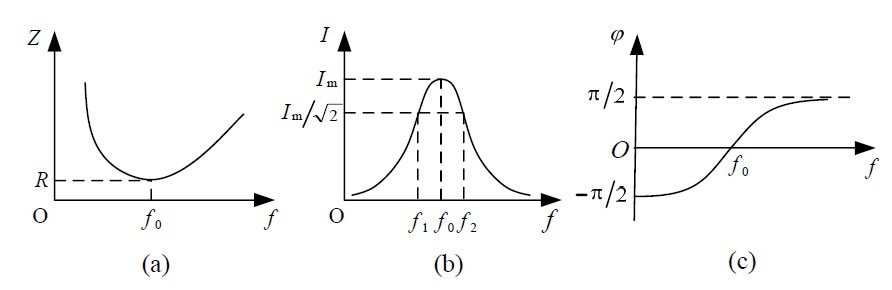
\includegraphics[scale=0.6]{fig5.jpg}
	\caption{The impedance, the current and the phase difference as functions of the frequency for a RLC series circuit (generic sketches).}
\end{figure}
\subsubsection{Quality Factor in Resonant Circuits}
Since Im = U/R, the voltages across the resistor, the inductor, and the capacitor are
$$ U_R=I_mR=U $$
$$ U_L=I_mZ_L=\dfrac{U}{R}\omega L $$
respectively. For a circuit driven at the resonance frequency, the ratio of $ U_L $ (or $ U_C $) to U is called the quality factor Q of a resonant circuit
$$ Q=\dfrac{U_L}{U}=\dfrac{\omega_0 L}{R}\text{  or  } Q=\dfrac{U_C}{U}=\dfrac{1}{\omega_0RC} $$

When the total voltage is fixed, the greater Q is, the greater $ U_L $ and $ U_C $ are. The value of Q can be used to quantify the effciency of resonant circuits.\\

The quality factor can also be found as
$$ Q=\dfrac{f_0}{f_2-f_1} $$
where $ f_1 $ and $ f_2 $ are two frequencies such that $ I(f_1) = I(f_2) = I_m/\sqrt{2} $ (see Figure 5b).

\section{Measurement Setup and Procedure}

\subsection{Apparatus}
The measurement setup consists of the following main elements: a signal generator, an oscilloscope, a digital multimeter, a wiring board, a fixed resistor $ 100\Omega (2 W) $, a variable resistor $ 2 k\Omega(2 W) $, two capacitors $ 0.47 \mu F $ and $ 0.1 \mu F $, as well as two inductors (10 mH and 33 mH).

\subsection{Measurement Procedure}
\subsubsection{RC, RL Series Circuit}

\begin{enumerate}
\item 
Choose a capacitor and an inductor to assemble a circuit with the fixed-resistance 100 resistor. Adjust the output frequency of the square-wave signal provided by the signal generator. Observe the change of the waveform (curve shown on the oscilloscope screen) when the time constant is smaller or greater than the half-period of the square wave. Use the PRINT function of the oscilloscope to record the waveforms.
\item 
Adjust display parameters of the oscilloscope and measure $ T_{1/2} $ for the studied circuits. Then, calculate the time constant and compare it with the theoretical value.In order to find the time constant accurately, only one period should be displayed on the oscilloscope screen.
\end{enumerate}

\subsubsection{RLC Series Circuit}

\begin{enumerate}
\item 
Choose a capacitor and an inductor to assemble a RLC series circuit with the variable resistor. Observe the waveform of the capacitor voltage in the underdamped, critically damped, and overdamped regimes. Use the PRINT function of the oscilloscope to store the waveforms.
\item 
Adjust the variable resistor to the critically damped regime. According to the definition of the half-life period $ T_{1/2} $, we have $ T_{1/2} = 1.68 $. By finding the value of $ T_{1/2} $, the time constant can be found as $ \tau = 1/\beta = T_{1/2}/1.68 $. Compare your result with the theoretical value.
\end{enumerate}

\subsubsection{RLC Resonant Circuit}
Apply a sinusoidal input voltage $ U_i $ to the RLC series circuit, change the frequency, then observe the change of the voltage $ U_R $ for a fixed resistor R, as well as the phase difference between $ U_R $ and $ U_i $. Measure how $ U_R $ changes with $ U_i $ and calculate the phase difference according to Figure 4. Plot the graphs $ f/f_0 $ vs. $ I/I_m $ and $ f/f_0 $ vs.$ \phi $. Estimate the resonance frequency and calculate the quality factor $ Q $.



\section{Results}

\subsection{RC, RL Series Circuit}

The measurement of a RC series circuit was shown in Table \ref{tab-1}.

\begin{table}[!h]
\begin{center}
\begin{tabular}{|c|c|}
\hline
$R$ [$\Omega$] $\pm$ 0.01 [$\Omega$]	&	96.95	\\
\hline
$f$ [$Hz$] $\pm$ 0.001 [$Hz$]	&	1000	\\
\hline
$\varepsilon$ [$Vpp$] $\pm$ 0.001 [$Vpp$]	&	4	\\
\hline
$C$ [$nF$] $\pm$ 0.01 [$nF$]	&	102.45	\\
\hline
$T_{1/2}$ [$\mu s$] $\pm$ 0.001 [$\mu s$]	&	6.800	\\
\hline
\end{tabular}
\caption{$T_{1/2}$ measurement data for a RC series circuit.}
\label{tab-1}
\end{center}
\end{table}

$$\tau_{theorem}=RC=9.933\pm0.0014\,\rm{\mu s}$$
$$\tau_{experiment}=\frac{T_{1/2}}{\ln 2}=9.810\pm0.0014\,\rm{\mu s}$$

The images printed in the experiment was shown in Figure \ref{fig-1}.

\begin{figure}[H]
	\centering
	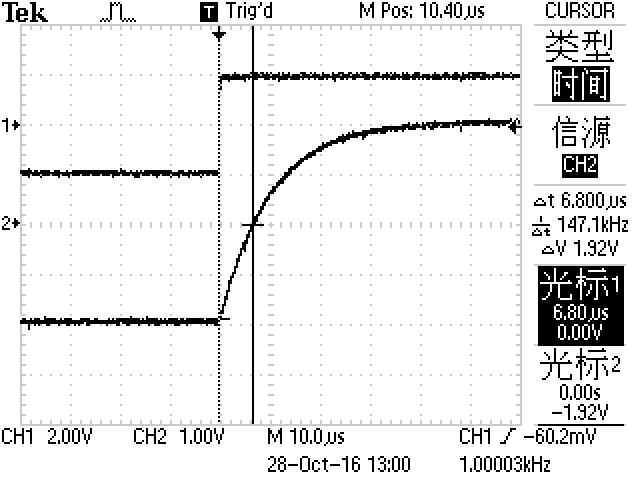
\includegraphics[scale=0.6]{TEK0002.jpg}
	\caption{RC circuit.}
	\label{fig-1}
\end{figure}

The measurement of a RL series circuit was shown in Table \ref{tab-2}.

\begin{table}[!h]
\begin{center}
\begin{tabular}{|c|c|}
\hline
$R$ [$\Omega$] $\pm$ 0.01 [$\Omega$]	&	96.95	\\
\hline
$f$ [$Hz$] $\pm$ 0.001 [$Hz$]	&	1000	\\
\hline
$\varepsilon$ [$Vpp$] $\pm$ 0.001 [$Vpp$]	&	4	\\
\hline
$L$ [$H$] $\pm$ 0 [$H$]	&	0.01	\\
\hline
$T_{1/2}$ [$\mu s$] $\pm$ 0.01 [$\mu s$]	&	68.00	\\
\hline
\end{tabular}
\caption{$T_{1/2}$ measurement data for a RL series circuit.}
\label{tab-2}
\end{center}
\end{table}

$$\tau_{theorem}=\frac{L}{R}=103.15\pm 0.01\,\rm{\mu s}$$
$$\tau_{experiment}=\frac{T_{1/2}}{\ln 2}=98.10\pm0.014\,\rm{\mu s}$$

The images printed in the experiment was shown in Figure \ref{fig-2}.

\begin{figure}[H]
	\centering
	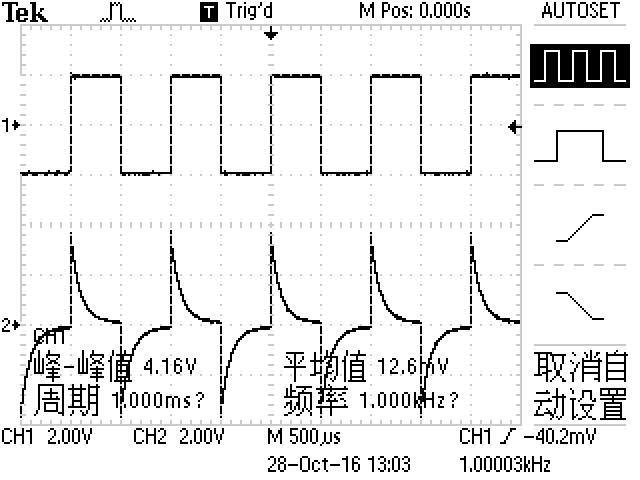
\includegraphics[scale=0.6]{TEK0003.jpg}
	\caption{RL circuit.}
	\label{fig-2}
\end{figure}

\subsection{RLC Series Circuit}

The measurement of a RLC series circuit was shown in Table \ref{tab-3}.

\begin{table}[!h]
\begin{center}
\begin{tabular}{|c|c|}
\hline
$L$ [$H$] $\pm$ 0 [$H$]	&	0.01	\\
\hline
$C$ [$nF$] $\pm$ 0.01 [$nF$]	&	102.45	\\
\hline
$f$ [$Hz$] $\pm$ 0.001 [$Hz$]	&	500	\\
\hline
$\varepsilon$ [$Vpp$] $\pm$ 0.001 [$Vpp$]	&	4	\\
\hline
$T_{1/2}$ [$\mu s$] $\pm$ 0.01 [$\mu s$]	&	56.00	\\
\hline
\end{tabular}
\caption{$T_{1/2}$ measurement data for a critically damped RLC series circuit.}
\label{tab-3}
\end{center}
\end{table}

$$\tau_{theorem}=\frac{1}{\beta}=\sqrt{LC}=32.078\pm0.006\,\rm{\mu s}$$
$$\tau_{experiment}=\frac{T_{1/2}}{1.68}=33.33\pm0.006\,\rm{\mu s}$$

The images printed in the experiment were shown in Figure \ref{fig-3}.

\begin{figure}[!h]
  \centering 
  \subfigure[Underdamped]{ 
    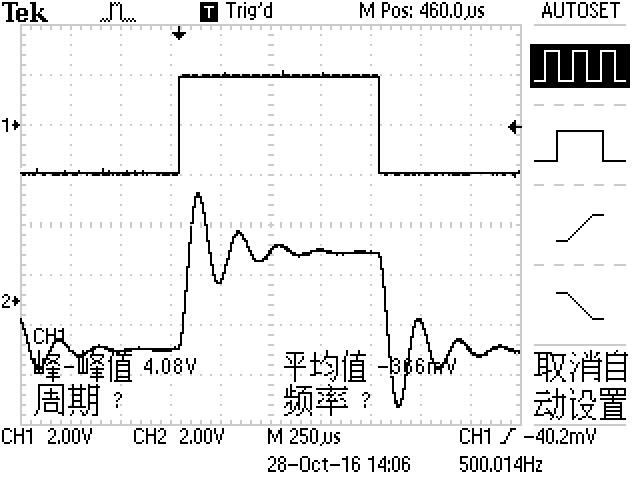
\includegraphics[width=1.5in]{TEK0005.jpg}} 
  \hspace{0.3in} 
  \subfigure[Critical Damped]{ 
    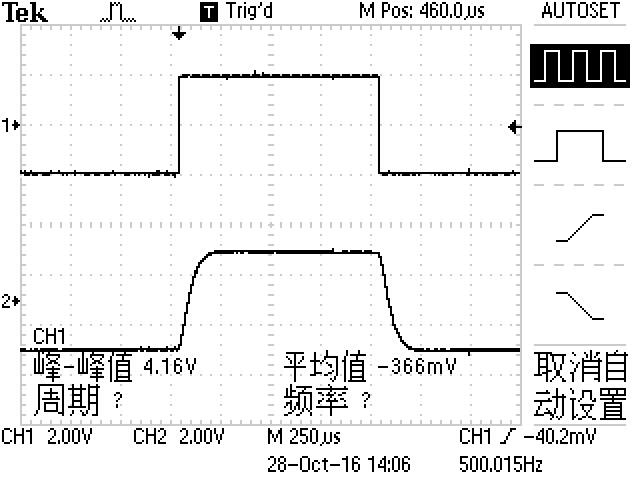
\includegraphics[width=1.5in]{TEK0006.jpg}} 
  \hspace{0.3in}   
  \subfigure[Overdamped]{ 
    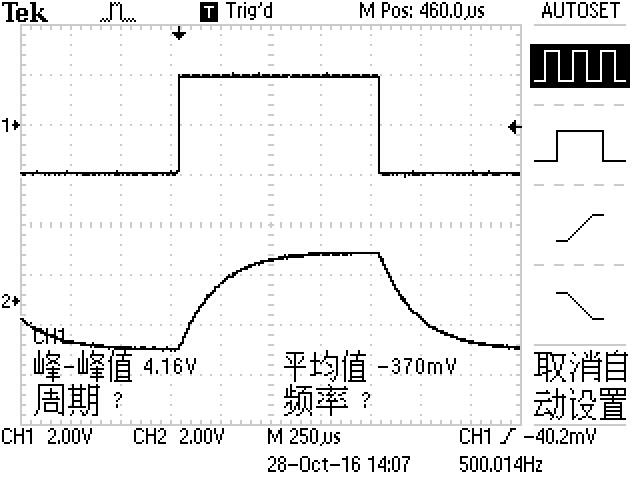
\includegraphics[width=1.5in]{TEK0007.jpg}} 
  \caption{RLC circuit.} 
  \label{fig-3}
\end{figure}

\subsection{RLC Resonant Circuit}

The measurement of a RLC resonant circuit was shown in Table \ref{tab-4}.

\begin{table}[H]
\centering
\begin{tabular}{|c|c|c|c|}
\hline
\multicolumn{2}{|c|}{$R$ [$\Omega$] $\pm$ 0.01 [$\Omega$]}	&	\multicolumn{2}{|c|}{96.95}	\\
\hline
\multicolumn{2}{|c|}{$L$ [$H$] $\pm$ 0 [$H$]}	&	\multicolumn{2}{|c|}{0.01}	\\
\hline
\multicolumn{2}{|c|}{$C$ [$nF$] $\pm$ 0.01 [$nF$]}	&	\multicolumn{2}{|c|}{102.45}	\\
\hline
\multicolumn{2}{|c|}{$f_0$ [$Hz$] $\pm$ 0.001 [$Hz$]}	&	\multicolumn{2}{|c|}{5032}	\\
\hline
\multicolumn{2}{|c|}{$\varepsilon$ [$Vpp$] $\pm$ 0.001 [$Vpp$]}	&	\multicolumn{2}{|c|}{4}	\\
\hline
& $U_R$ [$mV$] $\pm$ 10 [$mV$] & $f$ [$Hz$] $\pm$ 0.001 [$Hz$] & $\phi$ [$rad$]\\
\hline
1	&	132	&	500.000	&	$-1.539\pm0.000$	\\
\hline
2	&	268	&	1000.000	&	$-1.506\pm0.000$	\\
\hline
3	&	416	&	1500.000	&	$-1.468\pm0.000$	\\
\hline
4	&	608	&	2000.000	&	$-1.423\pm0.000$	\\
\hline
5	&	816	&	2500.000	&	$-1.365\pm0.000$	\\
\hline
6	&	1160	&	3000.000	&	$-1.285\pm0.000$	\\
\hline
7	&	1580	&	3500.000	&	$-1.162\pm0.000$	\\
\hline
8	&	2320	&	4000.000	&	$-0.955\pm0.000$	\\
\hline
9	&	2680	&	4250.000	&	$-0.793\pm0.000$	\\
\hline
10	&	3160	&	4500.000	&	$-0.572\pm0.000$	\\
\hline
11	&	3600	&	4750.000	&	$-0.287\pm0.000$	\\
\hline
12	&	3800	&	5000.000	&	$0.036\pm0.000$	\\
\hline
13	&	3680	&	5250.000	&	$0.337\pm0.000$	\\
\hline
14	&	3360	&	5500.000	&	$0.577\pm0.000$	\\
\hline
15	&	2920	&	5750.000	&	$0.754\pm0.000$	\\
\hline
16	&	2680	&	6000.000	&	$0.883\pm0.000$	\\
\hline
17	&	2080	&	6500.000	&	$1.051\pm0.000$	\\
\hline
18	&	1680	&	7000.000	&	$1.152\pm0.000$	\\
\hline
19	&	1440	&	7500.000	&	$1.219\pm0.000$	\\
\hline
20	&	1280	&	8000.000	&	$1.266\pm0.000$	\\
\hline
21	&	1140	&	8500.000	&	$1.302\pm0.000$	\\
\hline
22	&	992	&	9000.000	&	$1.329\pm0.000$	\\
\hline
\end{tabular}
\caption{Measurement data for the $U_R$ vs. $f$ dependence for a RLC resonant circuit.}
\label{tab-4}
\end{table}

The images analyzed were plotted in MATLAB and shown in Figure \ref{fig-4-1}. and Figure \ref{fig-4-2}. below.\\

The uncertainty of the two plots are too small so that it can't be displayed.

\begin{figure}[H]
	\centering
	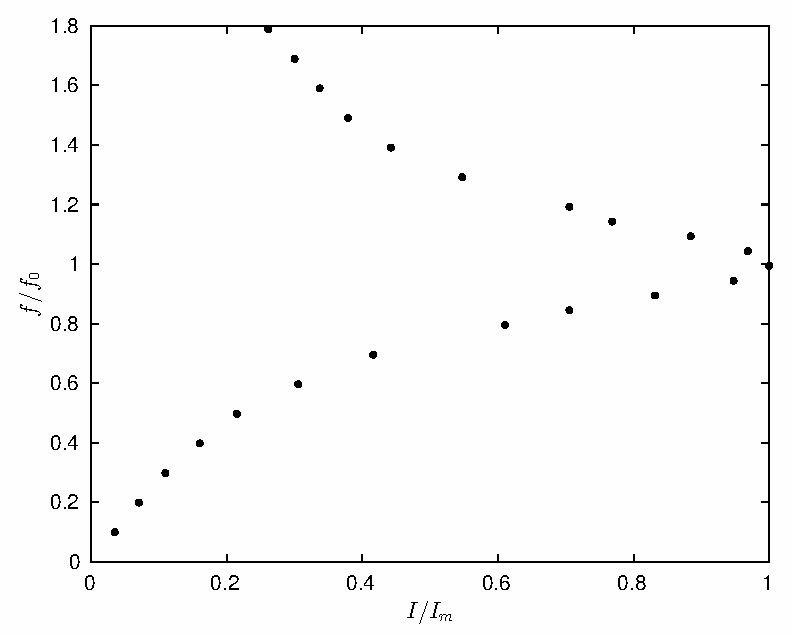
\includegraphics[scale=0.6]{4_1.eps}
	\caption{$f/f_0$ vs. $I/I_m$.}
	\label{fig-4-1}
\end{figure}

\begin{figure}[H]
	\centering
	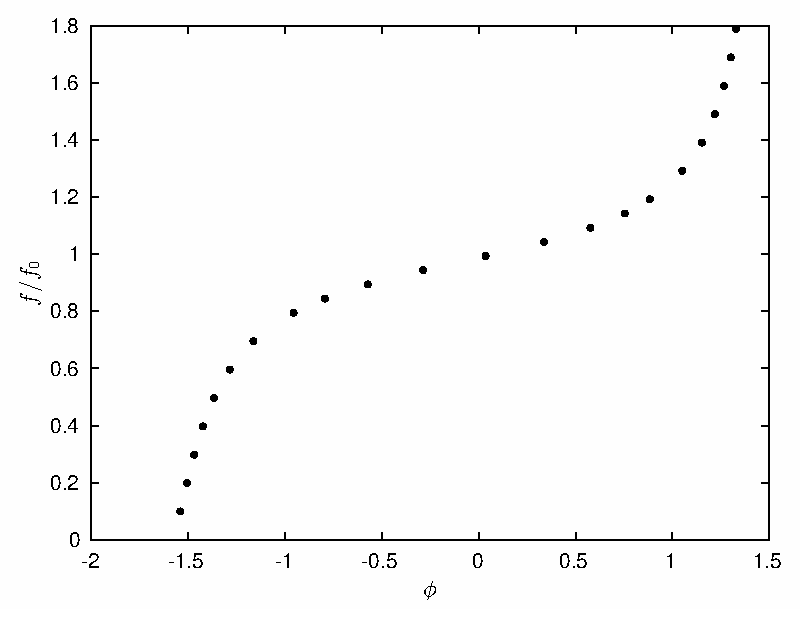
\includegraphics[scale=0.6]{4_2.eps}
	\caption{$f/f_0$ vs. $\phi$.}
	\label{fig-4-2}
\end{figure}

$$f_0=5032\,\rm{Hz}$$
$$Q=\frac{\omega_0L}{R}=3.26\pm0.00$$

\section{Measurement uncertainty analysis}

\subsection{theorem value of $\tau$}

The theorem value of $\tau$ in a RC series circuit can be calculated by the equation $\tau=RC$. Therefore its uncertainty $u_{\tau}$ is found by applying the uncertainty propagation formula

\begin{align*}
u_{\tau}&=\sqrt{\left(\frac{\partial \tau}{\partial R}\right)^2u_R^2+\left(\frac{\partial \tau}{\partial C}\right)^2u_C^2}\\
&=\sqrt{C^2u_R^2+R^2u_C^2}\\
&=1.41\times10^{-3}\,\rm{\mu s}
\end{align*}

The theorem value of $\tau$ in a RL series circuit can be calculated by the equation $\tau=\frac{L}{R}$. Therefore its uncertainty $u_{\tau}$ is found by applying the uncertainty propagation formula

\begin{align*}
u_{\tau}&=\sqrt{\left(\frac{\partial \tau}{\partial L}\right)^2u_L^2+\left(\frac{\partial \tau}{\partial R}\right)^2u_R^2}\\
&=\sqrt{\left(\frac{1}{R}\right)^2u_L^2+\left(\frac{L}{R^2}\right)^2u_R^2}\\
&=1.064\times10^{-2}\,\rm{\mu s}
\end{align*}

The theorem value of $\tau$ in a RLC series circuit can be calculated by the equation $\tau=\sqrt{LC}$. Therefore its uncertainty $u_{\tau}$ is found by applying the uncertainty propagation formula

\begin{align*}
u_{\tau}&=\sqrt{\left(\frac{\partial \tau}{\partial L}\right)^2u_L^2+\left(\frac{\partial \tau}{\partial C}\right)^2u_C^2}\\
&=\sqrt{\left(\sqrt{\frac{C}{4L}}\right)^2u_L^2+\left(\sqrt{\frac{L}{4C}}\right)^2u_C^2}\\
&=6.248\times10^{-3}\,\rm{\mu s}
\end{align*}

\subsection{experimental value of $\tau$}

The uncertainty of experimental value of $\tau$ can be simply calculated by directed divide a coefficient.\\

$u_{\tau}$ in a RC circuit is $0.001/\ln2=0.0014\,\rm{\mu s}$\\

$u_{\tau}$ in a RL circuit is $0.01/\ln2=0.014\,\rm{\mu s}$\\

$u_{\tau}$ in a RLC circuit is $0.01/1.68=0.006\,\rm{\mu s}$\\

\subsection{the phase $\phi$}

The phase $\phi$ in a RLC resonant circuit can be calculated by the equation $\phi=tan^{-1}\left(\dfrac{\omega L-\frac{1}{\omega C}}{R}\right)$. Therefore its uncertainty $u_{\phi}$ is found by applying the uncertainty propagation formula

\begin{align*}
u_{\phi}&=\sqrt{\left(\frac{\partial \phi}{\partial L}\right)^2u_L^2+\left(\frac{\partial \phi}{\partial C}\right)^2u_C^2+\left(\frac{\partial \phi}{\partial R}\right)^2u_R^2+\left(\frac{\partial \phi}{\partial \omega}\right)^2u_\omega^2}\\
&=\frac{1}{1+\left(\frac{\omega L-\frac{1}{\omega C}}{R}\right)^2}\sqrt{\left(\frac{\omega}{R}\right)^2u_L^2+\left(\frac{1}{\omega RC^2}\right)^2u_C^2+\left(\frac{\omega L-\frac{1}{\omega C}}{R^2}\right)^2u_R^2+\left(\frac{L}{R}-\frac{1}{\omega^2RC}\right)^2u_\omega^2}
\end{align*}

\subsection{The quality factor $Q$}

The theorem value of $Q$ in a RL series circuit can be calculated by the equation $Q=\frac{\omega_0 L}{R}$. Therefore its uncertainty $u_Q$ is found by applying the uncertainty propagation formula

\begin{align*}
u_{Q}&=\sqrt{\left(\frac{\partial Q}{\partial \omega_0}\right)^2u_{\omega_0}^2+\left(\frac{\partial Q}{\partial L}\right)^2u_L^2+\left(\frac{\partial Q}{\partial R}\right)^2u_R^2}\\
&=\sqrt{\left(\frac{L}{R}\right)^2u_{\omega_0}^2+\left(\frac{\omega_0}{R}\right)^2u_L^2+\left(\frac{\omega_0L}{R^2}\right)^2u_R^2}\\
&=3.36\times10^{-4}
\end{align*}

\section{Conclusion}
In this experiment, we understand the physics of alternating-current circuits, in particular the processes of charging/discharging of capacitors, the phenomenon of electromagnetic induction in inductive elements, and other dynamic processes in RC, RL, and RLC series circuits. Moreover, methods for measuring the amplitude-frequency and the phase-frequency characteristics of RC, RL, and RLC series circuits will be studied. The resonance frequency of a RLC circuit as well as the quality factor of the circuit will be found from the amplitude-frequency curve.\\

In a RC series circuit, we can find
$$\tau=RC$$

In a RL series circuit, we can find
$$\tau=\frac{L}{R}$$

In a RLC series circuit critical damped , we can find
$$\tau=\sqrt{LC}$$

Then we discovered the RLC resonant circuit, which is similar to a simple harmonic oscillation. We plotted the experiment results in certain method so that we can find the property of it. We also calculated the The quality factor $Q$ within the theorem.

\section{Reference}

\begin{enumerate}[(a)]
	\item
	Qin Tian, Feng Yaming, Mateusz Krzyzosiak, VP241 Exercise 5, RC, RL, and RLC Circuits, based on materials provided by the Department of Physics, Shanghai Jiaotong University.
\end{enumerate}

\section{Data sheet}

The Data sheet is attached at the end of the report.

\end{document}
